\documentclass[a4paper,twoside,11pt]{scrartcl}
%encodings
\usepackage[utf8]{inputenc}
\usepackage[USenglish]{babel}
\usepackage[T1]{fontenc}
%colors, hyperrefs
\usepackage{color}
\usepackage{url}
\usepackage[pdftex,pdfauthor={J\"org Behrmann, Anika Haller},pdftitle={M2: Atomic Force Microscopy}]{hyperref}
%figures and subfigures
\usepackage[pdftex]{graphicx}
\usepackage{subfigure}
%better tables
\usepackage{tabularx}
\usepackage{booktabs}
%math stuff
\usepackage{amsmath}
\usepackage{amsthm}
\usepackage{amsfonts}
\usepackage{IEEEtrantools}
%shiny stuff
\usepackage[babel]{microtype}
\DisableLigatures{encoding=T1,family=tt*}

\begin{document}

\title{Atomic force microscopy}
\author{J\"org Behrmann \qquad Anika Haller}
\date{31.10.2011}
\maketitle
\tableofcontents
\thispagestyle{empty}
\clearpage

\section{Introduction and Physical Background}

The first kind of a wide variety of scanning probe microscopes (SPM) was invented in 1981 by Gerd Binnig and Heinrich Rohrer at IBM ZürichResearch, the Scanning Tunneling Microscope (STM). Its invention sparked the development of other SPMs that could address some of the STMs shortcomings. For example, relying on a tunneling current the STM can only be used with conducting materials (for probe and sample).
The first answers to those shortcomings was the Atomic Force Microscope (AFM), which was invented in 1986 by Binnig, Quate and Gerber.

All SPM techniques have in common that a measuring probe is moved by piezoelectric actuators in a raster over the sample. The difference between AFM and STM is that instead of using a tunneling current, the AFM uses a small cantilever that reacts to the interatomic forces between sample and cantilever tip. Thus the AFM can work with virtually any sample material, especially non-conducting materials that cannot be investigated with a STM. 

\subsection{Experimental Setup \label{sec:setup}}

A block diagram of an AFM can be found in figure \ref{fig:block}. The essential element is AFM head with the cantilever. The cantilever is small arm with a sharp tip. The cantilever is influenced by atomic and can be moved by piezoelectric actuators in all spatial directions. The movement of the cantilever is detected by its reflection of a laser beam on a photodiode.
The movement by the piecoelectric actuators can be coupled to a feedback loop so that the cantilever can be held at constant height over the sample or in a way that the force on the cantilever remains constant. This will be important for the different modes of operation of the AFM

\begin{figure}[ht]
\centering
\subfigure{
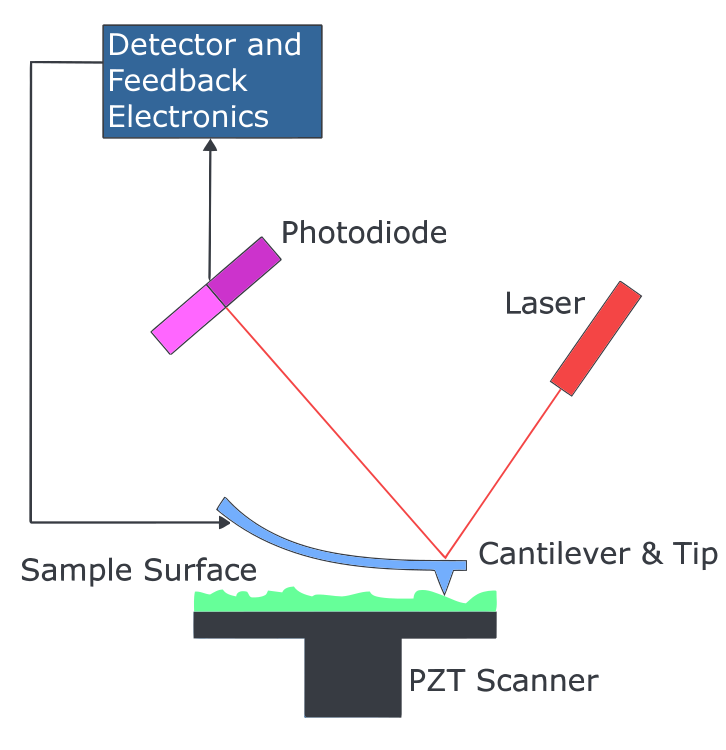
\includegraphics[scale=0.2]{img/Atomic_force_microscope_block_diagram}
\label{fig:block}
}
\subfigure{
\includegraphics[scale=0.40]{img/forces}
\label{fig:forces}
}
\caption{General AFM setup \subref{fig:block}, Forces on a cantilever tip \subref{fig:forces}}
\end{figure}

\subsection{Atomic Forces}

The tip of an AFM can approach a sample to within a few \AA so that its interaction with the sample is the sum of all imaginable atom forces
\begin{equation}
F_{a}=F_{ch}+F_{vdW}+F_{el}+F_{mag}.
\end{equation}

The chemical and van der Waals Forces $F_{ch}$ and $F_{vdW}$ can be modelled by the empirical Lennard-Jones potential
\begin{equation}
V_{ch}=4\epsilon\left[\left(\frac{\sigma_{0}}{r}\right)^{12}-\left(\frac{\sigma_{0}}{r}\right)^{6}\right],
\end{equation}
where the first term describes a strong short range repulsion, consisting of the Pauli repulsion of overlapping electron shells of the sample and the tip and the repulsion between the nuclei in the sample and the tip, whereas the second term describes the attraction through the van der Waals force, the attraction between non-permanent dipoles in atoms. In the context of atom force microscopy it can be modelled by
\begin{equation}
F_{vdW}=\frac{HR}{6d^{2}}
\end{equation}
where $R$ is the radius of the tip, $d$ is the sample-tip distance and $H$ is the Hamaker constant, which is only a constant in so far, that is constant for a combination of tip and sample, because it depends on the number of atoms per unit volume in the sample and the tip.

The Coulomb force $F_el$ follows from the contact potential
\begin{equation}
U_{contact}=\frac{1}{e}\left(\Phi_{tip}-\Phi_{sample}\right),
\end{equation}
where the $\Phi_i$ are the work functions of the respective materials. The combined system of sample and tip can be seen as a capacitor and the force is then given by the change in capacitance $C$. If an additional bias voltage is applied the force is given by
\begin{equation}
F_{el}=\frac{1}{2}(U_{bias}+U_{contact})^2 \label{eq:elec}
\end{equation}
This term will be explained more later, when we will talk about Kelvin Force Spectroscopy (KFS).

The magnetic force $F_{mag}$ is only relevant for magnetized tips on magnetic samples and will not concern us further.

The resulting forces over distance can be seen schematically in figure \ref{fig:forces}.

\subsection{Experimental Techniques}

\subsection{Modes of Operation}

\subsubsection{Contact AFM}

In Contact AFM the tip of the cantilever is kept in the region of strong repulsion, as seen in figure \ref{fig:forces}. The cantilever can be moved over the sample in two different modes: \textit{constant height} and \textit{constant force}.

In constant height mode the cantilever is moved over the sample with a constant height above the sample, and the spatial variations in the atomic forces flex the cantilever, which can be measured optically as described in section \ref{sec:setup}.

In constant force mode the force acting on the cantilever is held constant by varying its height over the sample through a feedback loop.

Contact mode bears the risk that the tip of the cantilever might crash into the sample and contaminate it.

\subsubsection{Non-contact AFM}

In Non-contact AFM (nc-AFM) the tip of the cantilever is held far away from the sample in the attractive part of the potential in figure \ref{fig:forces}. Usually nc-AFM uses harder cantilever materials, with higher spring constants, so that the chance of crashing the tip into the sample is decreased.

Far away from the sample the atomic forces are very weak, so that the use of constant force mode is not feasible. The measurement is rather done by oscillating the cantilever at its resonance frequency.

The movement of the tip can be modelles as a damped, forced harmonic oscillator
\begin{equation}
m\ddot{z}+\gamma \dot{z}+kz=F_{0}e^{i\Omega t}+F_{a} \label{eq:differential}
\end{equation}
where $z$ is the sample-tip distance, $m$ is the mass, $\gamma$ is the damping factor, $k$ is the spring constant and $F_0$ is the amplitude of the driving force by the piecoelectric actuators. The oscillation frequence is given by $\omega_0\,=\,\sqrt{k/m}$. For a small amplitude of the oscillation in $z$, i.e. the tip remaining far away from the sample, we expand the atomic forces and keep only the linear term. The constant term shifts the equlibrium position of the oscillator and can be neglected, the linear term changes the spring constant
\begin{equation}
k_{eff}=k-\frac{\partial F_{a}}{\partial z} \label{eq:change},
\end{equation}
which shifts the resonance frequency accordingly (as can be easily seen by dividing \eqref{eq:change} by $m$ and expanding the squareroot)
\begin{equation}
\Delta \omega_0 = -\frac{1}{2} \frac{\omega-0}{k} \frac{\partial F_{a}}{\partial z}
\end{equation}

The shift in resonance frequency can be measured by a change in the amplitude of the cantilever oscillation. The change in amplitude can be found by inserting the exponential ansatz $z=A\exp\left(i\Omega t\right)$ \eqref{eq:differential}. We get
\begin{equation}
A=\frac{A_{0}}{i\gamma\Omega+\omega_{0}^{2}-\Omega^{2}},
\end{equation}
where $A_0=F_0/m$ is the amplitude of the oscillator without the driving force. This amplitude is a complex number. The phase can be interpreted as a phase shift, the magnitude is the amplitude we wanted:
\begin{equation}
|A|^{2}=\frac{a_{0}}{(\omega_{0}^{2}-\Omega^{2})^{2}+\gamma^{2}\Omega^{2}}=\frac{a_{0}}{(\omega_{0}^{2}-\Omega^{2})^{2}-\gamma(\omega_{0}^{2}-\Omega^{2})+\gamma^{2}\omega_{0}^{2}}.
\end{equation}

Introducing the quality factor of the cantilever $Q=\omega_0/2\gamma$ and the relative amplitude $a=A_0/A$ we can now calculate the Force gradient
\begin{equation}
\frac{\partial F_{a}}{\partial z}=k\left(\frac{1-2a^{2}+\sqrt{4Q^{2}\left(a^{2}-1\right)+1}}{2\left(Q^{2}-a^{2}\right)}\right)
\end{equation}

\subsection{Spectroscopy}

The STM can be used for severall spectroscopic techniques, as can be the AFM if the cantilever and sample are made of conducting materials

\subsubsection{Kelvin Force Spectroscopy}

The Kelvin method is a technique to measure the contact potential differences (CPD) between a reference electrode and a sample. The Coulomb force was given by \eqref{eq:elec} and is obviously quadratic in the voltages. The minimum of the force can be found by applying a bias voltage that exactly cancels the CPD.
This bias voltage can be found in constant height mode by measuring the amplitude against the bias voltage. A parabola can then be fitted in the resulting dataset giving the wanted information.

\subsubsection{In Situ Tip Characterization}

\textit{Olsson et al. (J. Appl. Phys., 84, 8, 1998)} proposed a technique to discover the size and shape of the cantilever tip. The capacitance in \eqref{eq:elec} changes with tip-sample seperation. Modelling the capacitor that is the tip-sample system as an infinite conducting plane against a certain geometric form, one can predict the sample-tip separation as a function of bias voltage, as seen in table \ref{tab:tipshape}. Naturally those measurements need to be done in constant-force mode.

\begin{table}
\begin{center}
\begin{tabular}{lccr}
\toprule
Model & $F$ & $F'$ & $d|_{F'\,=\,\mbox{const}}$ \\
\midrule
Sphere & $-\frac{\pi \epsilon_0 R U^2}{d}$ & $\frac{\pi \epsilon_0 R U^2}{d^2}$ & $\left(\frac{\pi \epsilon_0 R}{F'}\right)^{1/2} U^{\phantom{1/2}}$ \\
Charged line (cone) & $-\frac{\alpha^2}{4 \pi \epsilon_0} \ln\left(\frac{L}{4d}\right) U^2$ & $\frac{\alpha^2 U^2}{4 \pi \epsilon_0 d}$ & $\left(\frac{\alpha^2}{4 \pi \epsilon_0 F'}\right) U^{2\phantom{/3}}$ \\
Plane surface (circular area) & $-\frac{\pi \epsilon_0 R^2 U^2}{2 d^2}$ & $\frac{\pi \epsilon_0 R^2 U^2}{d^3}$ & $\left(\frac{\pi \epsilon_0 R^2}{F'}\right) U^{2/3}$\\
\bottomrule
\end{tabular}
\end{center}
\par
\caption{Analytical expressions for force and force gradient for different tip shape models \label{tab:tipshape}}
\end{table}

\end{document}